%%%%%%%%%%%%%%%%%%%%%%%%%%%%%%%%%%%%%%%%%%%%%%%%%%%%%%%%%
%
%    AGH University of Krakow Beamer Theme Presentation
%    Prezentacja systemu: System do śledzenia przebiegu eksperymentów labolatoryjnych
%    Autorzy: Oliwia Rewer, Paulina Wór, Mateusz Woźniak
%
% opis aplikacji - zastosowanie, użytkownicy, role,
% opis walidacji wprowadzanych danych,
% dane - skąd były wzięte i w jaki sposób zostały wprowadzane,
% omówienie wyglądu aplikacji - style CSS,
% dynamiczna zawartość - skrypty JS, generowanie mediów przez serwer,
% najciekawsze elementy aplikacji,
% sposób testowania aplikacji.
%
%
%%%%%%%%%%%%%%%%%%%%%%%%%%%%%%%%%%%%%%%%%%%%%%%%%%%%%%%%%

\documentclass[polish,aspectratio=1610]{beamer}
\usetheme[parttitle=date]{AGH} % Bez opcji 'dark' dla białego tła
\usepackage[utf8]{inputenc}
\usepackage[T1]{fontenc}
\usepackage{graphicx}
\usepackage{hyperref}
\usepackage[polish]{babel}

\title{Prezentacja systemu:\\System do śledzenia przebiegu eksperymentów labolatoryjnych}
\author{Rewer, Wór, Woźniak}

\date{}

\begin{document}

    \maketitle

%%%%%%%%%%%%%%%%%%%%%%%%%%%%%%%%%%%%%%%%%%%%%%


    \section{Wprowadzenie}
%%%%%%%%%%%%%%%%%%%%%%%%%%%%%%%%%%%%%%%%%%%%%%
    \begin{frame}{System BioPlatform}
        \begin{itemize}
            \item System do śledzenia eksperymentów laboratoryjnych dla zespołów badawczych
            \item Główne funkcje:
            \begin{itemize}
                \item Gromadzenie i wizualizacja danych pomiarowych
                \item Zarządzanie eksperymentami i zespołami
                \item Automatyczna analiza obrazów mikroskopowych
                \item Współpraca między naukowcami poprzez system ról
            \end{itemize}
            \item Zaimplementowany w Django z interfejsem Tailwind CSS
        \end{itemize}
    \end{frame}

%%%%%%%%%%%%%%%%%%%%%%%%%%%%%%%%%%%%%%%%%%%%%%


    \section{Panel użytkownika}
%%%%%%%%%%%%%%%%%%%%%%%%%%%%%%%%%%%%%%%%%%%%%%
    \begin{frame}{System BioPlatform}
        \begin{figure}
            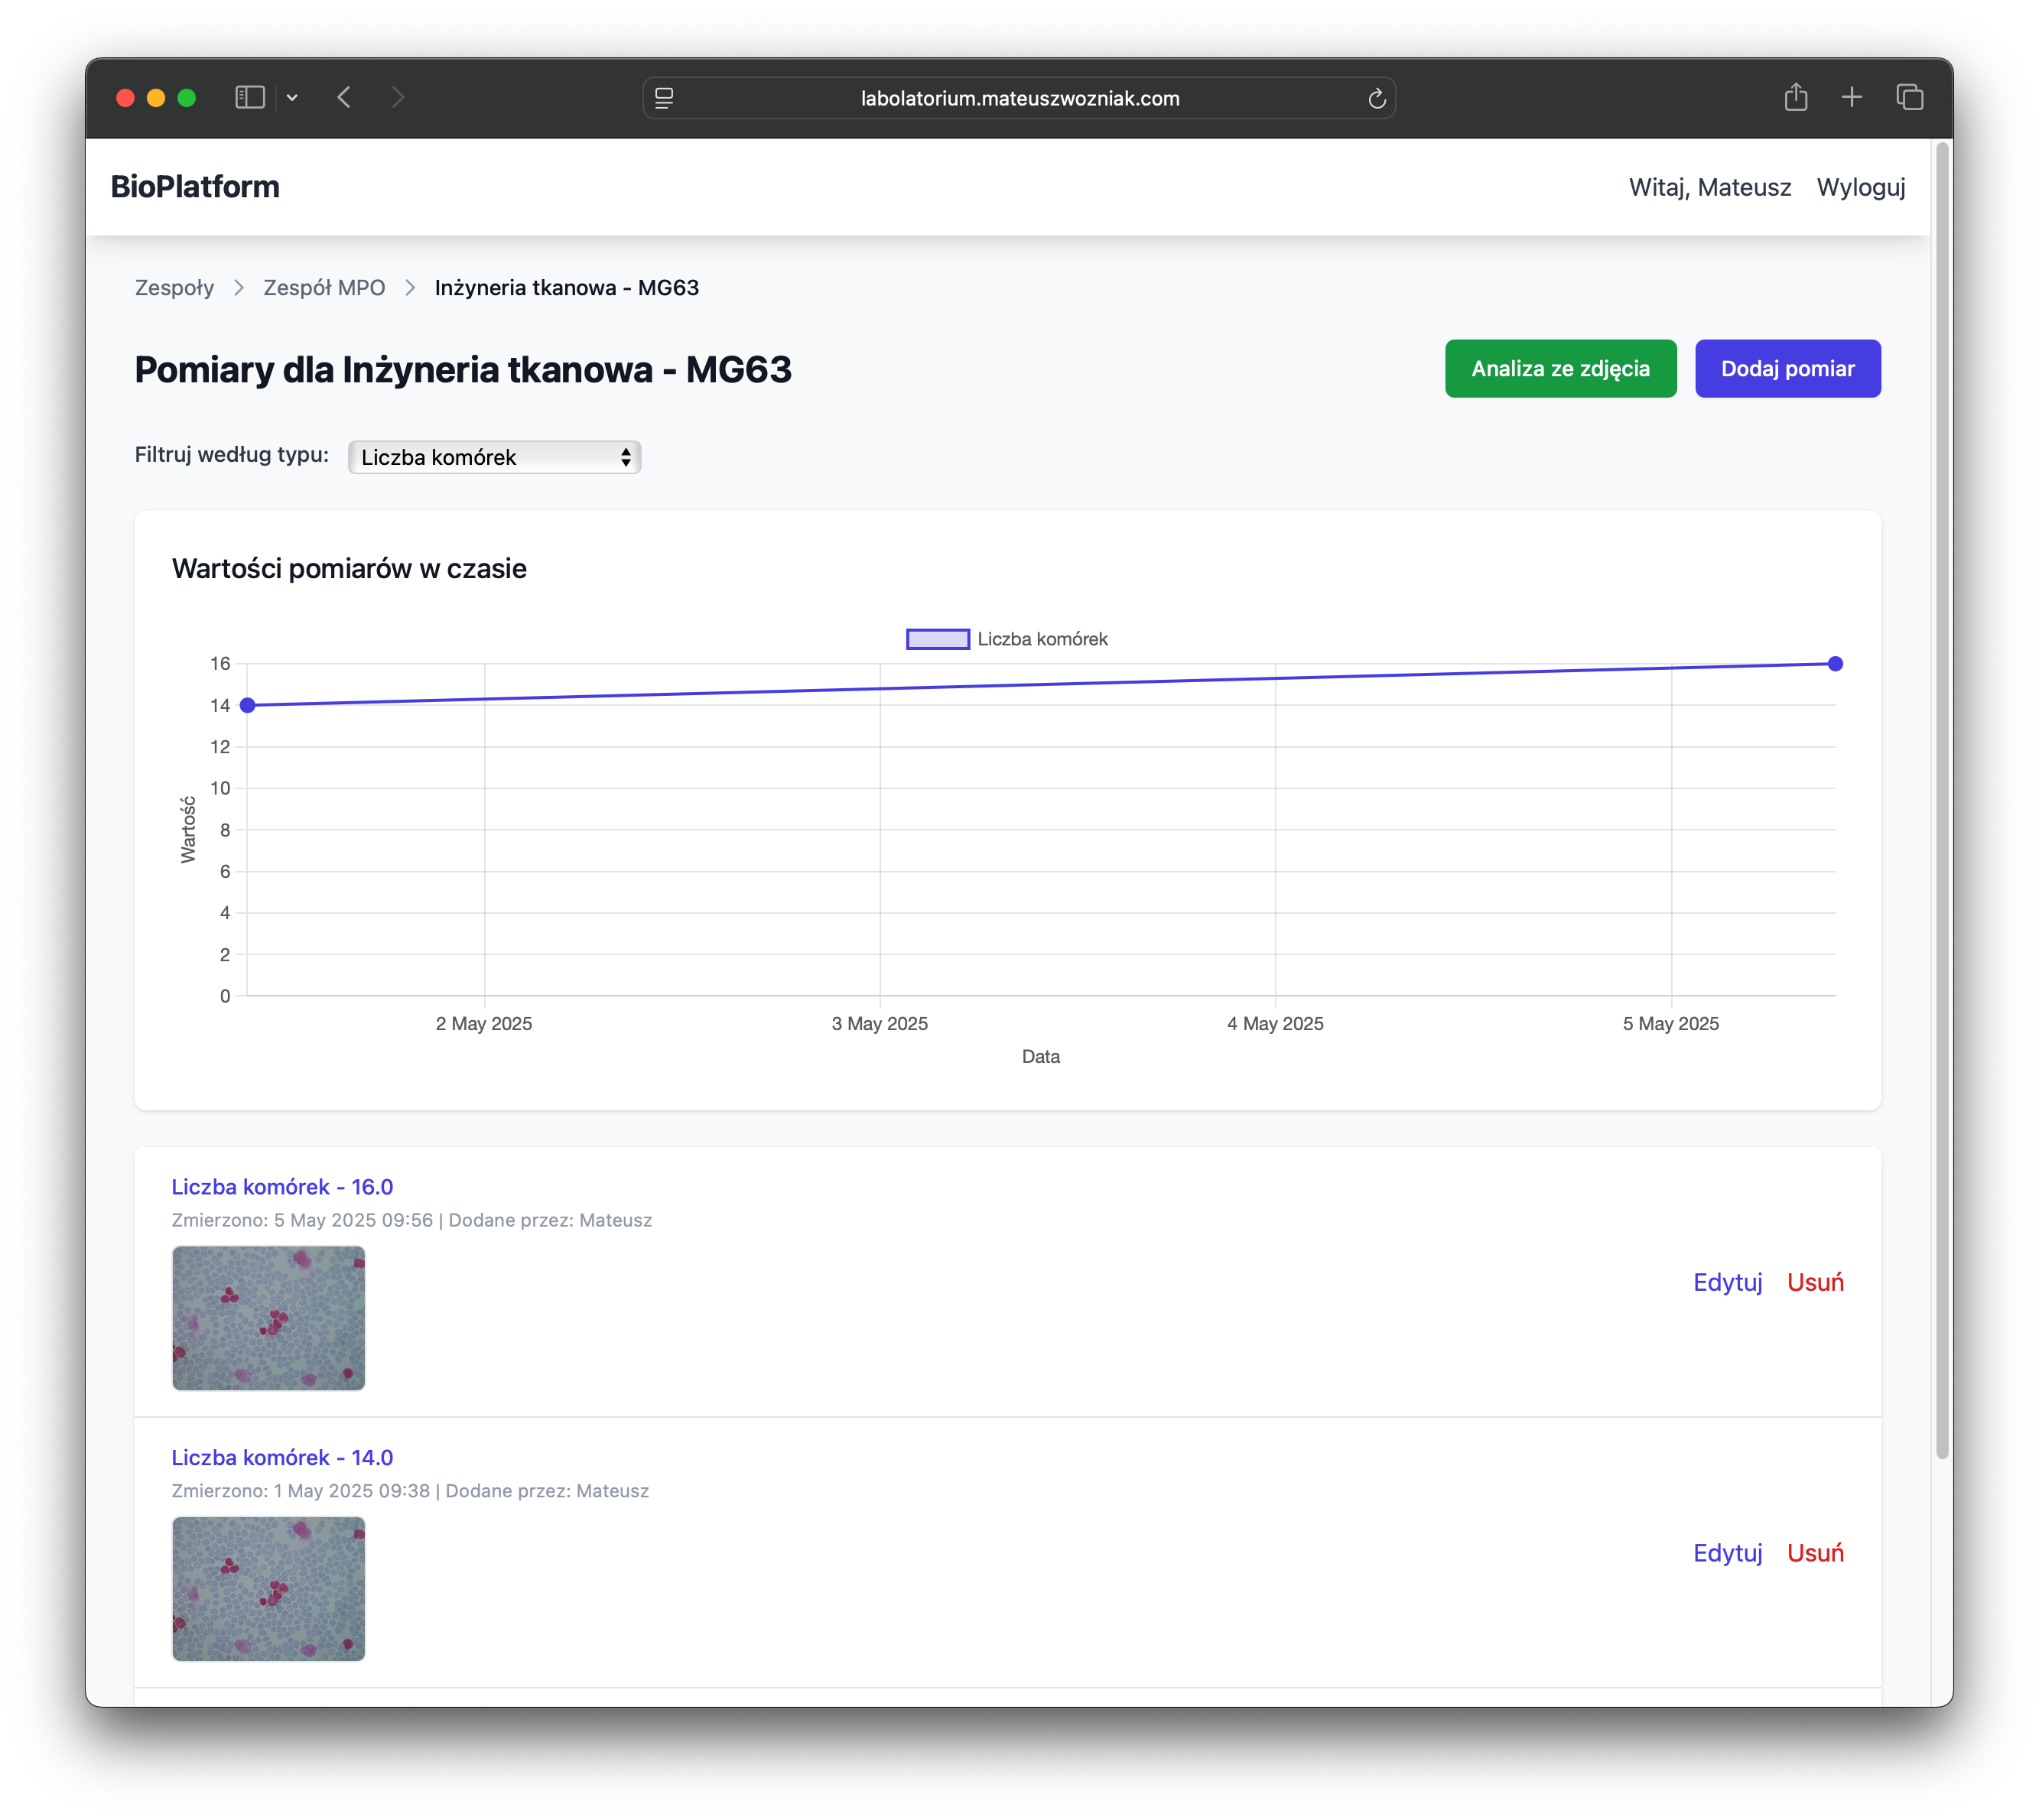
\includegraphics[width=0.8\textwidth]{screenshot.png}
        \end{figure}
    \end{frame}

%%%%%%%%%%%%%%%%%%%%%%%%%%%%%%%%%%%%%%%%%%%%%%
    \section{Role użytkowników}
%%%%%%%%%%%%%%%%%%%%%%%%%%%%%%%%%%%%%%%%%%%%%%
    \begin{frame}{Role w systemie BioPlatform}
        \begin{itemize}
            \item \textbf{Administrator (ADMIN)}
            \begin{itemize}
                \item Pełna kontrola nad zespołem
                \item Zarządzanie członkami zespołu (dodawanie, usuwanie, zmiana ról)
                \item Edycja i usuwanie zespołu
                \item Tworzenie, edycja i usuwanie eksperymentów oraz pomiarów
            \end{itemize}
            \item \textbf{Edytor (EDITOR)}
            \begin{itemize}
                \item Tworzenie, edycja i usuwanie eksperymentów w zespole
                \item Dodawanie, edycja i usuwanie pomiarów
                \item Brak możliwości zarządzania członkami zespołu
            \end{itemize}
            \item \textbf{Odczyt (VIEWER)}
            \begin{itemize}
                \item Przeglądanie eksperymentów i pomiarów
                \item Brak możliwości wprowadzania zmian
                \item Brak dostępu do zarządzania zespołem
            \end{itemize}
        \end{itemize}
    \end{frame}

%%%%%%%%%%%%%%%%%%%%%%%%%%%%%%%%%%%%%%%%%%%%%%
    \section{Walidacja danych}
%%%%%%%%%%%%%%%%%%%%%%%%%%%%%%%%%%%%%%%%%%%%%%
    \begin{frame}{Walidacja wprowadzanych danych}
        \begin{itemize}
            \item \textbf{Formularze Django:} Automatyczna walidacja pól modelu i formularza (np. wymagane pola, typy danych, unikalność).
            \item \textbf{Rejestracja użytkownika:}
            \begin{itemize}
                \item Sprawdzenie zgodności hasła i powtórzonego hasła
                \item Minimalna długość hasła (8 znaków)
                \item Unikalność e-maila i nazwy użytkownika
            \end{itemize}
            \item \textbf{Tworzenie/edycja zespołów, eksperymentów, pomiarów:}
            \begin{itemize}
                \item Wymagane pola (nazwa, opis, wartość)
                \item Ograniczenia typów danych (np. liczba dla wartości pomiaru)
                \item Walidacja typu pliku przy zdjęciach (tylko obrazy)
                \item Automatyczne ustawianie domyślnych wartości (np. data pomiaru)
            \end{itemize}
            \item \textbf{Role i uprawnienia:}
            \begin{itemize}
                \item Sprawdzanie uprawnień do operacji (np. tylko admin może usuwać zespół)
                \item Ograniczenie zmiany ról i usuwania ostatniego administratora
            \end{itemize}
            \item \textbf{Walidacja po stronie serwera:} Każda operacja zapisu jest weryfikowana po stronie serwera a nie aplikacji klienta.
        \end{itemize}
    \end{frame}

\end{document}
